\section{Resultados}

Os resultados obtidos nos testes de validação apresentam a média dos valores coletados após diversas execuções dos quatro testes de mudança de forma sequencial em uma máquina virtual. Tanto o serviço SWAPI como os clientes JavaScript foram executados no mesmo ambiente computacional, porém com conexão local de latência 10Mbps para simulação de um ambiente distribuído. Para a variável de processamento, foram utilizados valores que pudessem representar um dispositivo computacional de médio porte contando com 1 CPU de 2.4 GHz e 4Gb de RAM.

Inicialmente, observa-se na figura 26 que o cliente 1 (sem o uso da ferramenta) não apresenta um bom índice de acerto das respostas. Dentre as quatro mudanças, obteve apenas 58\% de acerto, sendo a C3 a única mudança em que conseguiu responder corretamente todas as perguntas, pois não houve mudança nas URIs que estava utilizando. Um resultado esperado, significando que houve quebra de contrato e impacto negativo no código de busca.

Em contrapartida, o cliente 2 (com o uso da ferramenta) apresenta um resultado no índice de acerto da figura 27 36.61\% superior ao cliente 1. Com um total de 91,5\% de acerto, apenas não completou com 100\% de acerto pois a mudança C4 não permitiu que fosse possível acessar todos os dados necessários para a responder da pergunta Q2. Isso representa que a ferramenta foi capaz, através do intermediador, de evitar a criação de contrato e causar impacto negativo ao código de busca.

Nota-se que ambos os clientes não apresentaram erros na resposta, porém acabam não respondendo pois ocorrem exceções durante o código de busca ou na lógica do cliente devido ao impacto das mudanças no fluxo de dados.

\begin{figure}[H]
  \centering
  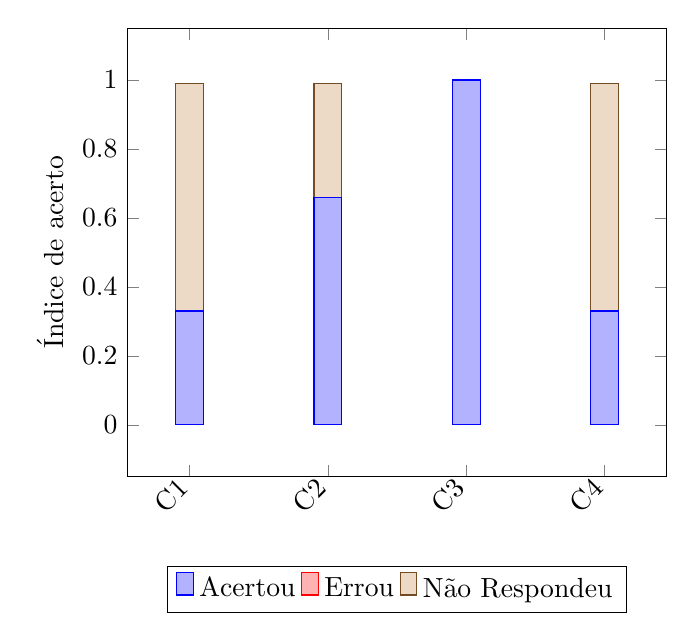
\begin{tikzpicture}
  \begin{axis}[
      ybar stacked,
      ymax=1,
      ymin=0,
      enlargelimits=0.15,
      legend style={at={(0.5,-0.20)},
        anchor=north,legend columns=-1},
      ylabel={Índice de acerto},
      symbolic x coords={C1, C2, C3, C4,
          C5, C6, C7},
      xtick=data,
      x tick label style={rotate=45,anchor=east},
      ]
  \addplot+[ybar] plot coordinates {(C1,0.33) (C2,0.66)
    (C3,1) (C4,0.33)};
  \addplot+[ybar] plot coordinates {(C1,0) (C2,0)
    (C3,0) (C4,0)};
  \addplot+[ybar] plot coordinates {(C1,0.66) (C2,0.33)
    (C3,0) (C4,0.66)};
  \legend{Acertou, Errou, Não Respondeu}
  \end{axis}
  \end{tikzpicture}
  \caption{Índice de acerto sem o uso da ferramenta}
\end{figure}

\begin{figure}[H]
  \centering
  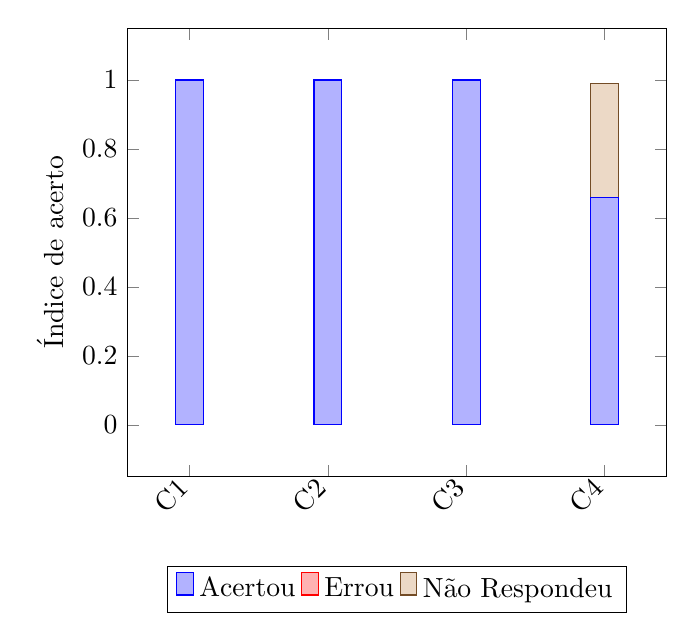
\begin{tikzpicture}
  \begin{axis}[
      ybar stacked,
      ymax=1,
      ymin=0,
      enlargelimits=0.15,
      legend style={at={(0.5,-0.20)},
        anchor=north,legend columns=-1},
      ylabel={Índice de acerto},
      symbolic x coords={C1, C2, C3, C4,
          C5, C6, C7},
      xtick=data,
      x tick label style={rotate=45,anchor=east},
      ]
  \addplot+[ybar] plot coordinates {(C1,1) (C2,1)
    (C3,1) (C4,0.66)};
  \addplot+[ybar] plot coordinates {(C1,0) (C2,0)
    (C3,0) (C4,0)};
  \addplot+[ybar] plot coordinates {(C1,0) (C2,0)
    (C3,0) (C4,0.33)};
  \legend{Acertou, Errou, Não Respondeu}
  \end{axis}
  \end{tikzpicture}
  \caption{Índice de acerto com o uso da ferramenta}
\end{figure}

Ao analisar a mudança C3 isoladamente, onde ambos conseguem responder com 100\% de acerto, percebe-se nas figuras 28 e 29 que o cliente 2 consegue realizar uma consulta com melhor desempenho (menor número de requisições e tamanho de dados) que o cliente 1. Isso porque, após a mudança e sem alterar o código de busca de dados, a ferramenta consegue remapear as requisições geradas pelas consultas GraphQL graças ao algoritmo que automatiza as chamadas à API.

Outro ponto importante é que, após a mudança C3 e a atualização dos metadados no cliente, o algoritmo da ferramenta percebe que há a possibilidade de realizar menos requisições em busca dos dados para responder as perguntas. Isso resulta em uma redução de aproximadamente 54\% dos acessos entre o cliente 1 e cliente 2.

\begin{figure}[H]
  \centering
  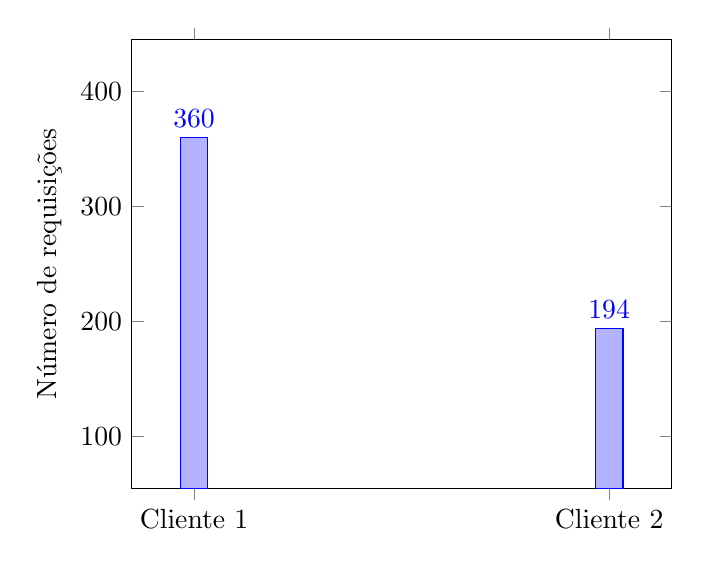
\begin{tikzpicture}
  \begin{axis}[
      ybar,
      ymax=400,
      ymin=100,
      enlargelimits=0.15,
      ylabel={Número de requisições},
      symbolic x coords={Cliente 1,Cliente 2},
      xtick=data,
      nodes near coords,
      nodes near coords align={vertical},
      ]
  \addplot coordinates {(Cliente 1,360) (Cliente 2,194)};
  \end{axis}
  \end{tikzpicture}
  \caption{Comparação no número de requisições C3}
\end{figure}

\begin{figure}[H]
  \centering
  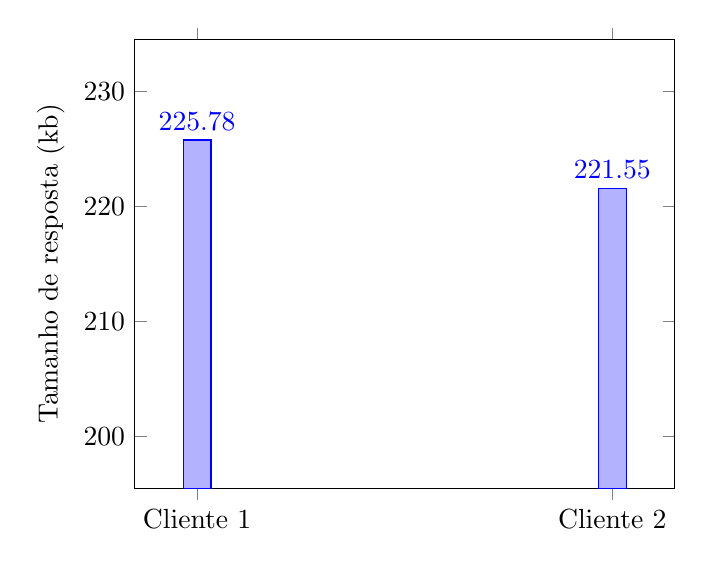
\begin{tikzpicture}
  \begin{axis}[
      ybar,
      ymax=230,
      ymin=200,
      enlargelimits=0.15,
      ylabel={Tamanho de resposta (kb)},
      symbolic x coords={Cliente 1,Cliente 2},
      xtick=data,
      nodes near coords,
      nodes near coords align={vertical},
      ]
  \addplot coordinates {(Cliente 1,225.777) (Cliente 2,221.547)};
  \end{axis}
  \end{tikzpicture}
  \caption{Comparação no tamanho de resposta C3}
\end{figure}

Apesar dos ganhos de performance e desenvolvimento através do uso da ferramenta vistos anteriormente, percebe-se na figura 30 um outro cenário que indica o lado negativo do seu uso causado pelo tempo de \textit{overhead}\footnote{
  Processamento em excesso
}. Em média, a ferramenta atrasou em 1.7 segundos a execução na consulta de dados do cliente, sendo o tempo de busca de metadados responsável por somar mais da metade deste atraso inicial.

Contudo, é importante levar em consideração que este tempo de \textit{overhead} é um impasse relativo ao tempo de vida do cliente que está sendo executado. Por exemplo, em clientes com tempo de vida curto ou que dependem de carregamento rápido, a ferramenta pode não ser a solução ideal. Nos demais casos, são visíveis os benefícios que seu uso pode trazer.

\begin{figure}[H]
  \centering
  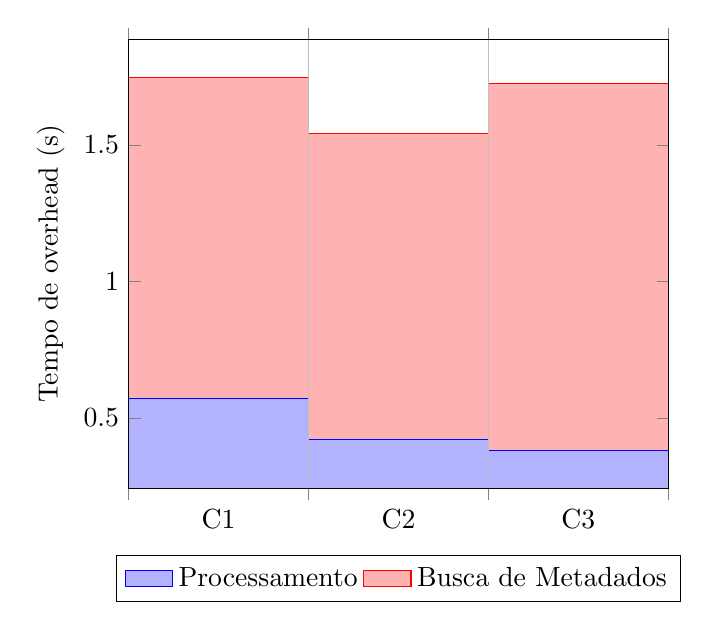
\begin{tikzpicture}
	\begin{axis}[
        ybar interval,
        ylabel={Tempo de overhead (s)},
        legend style={at={(0.5,-0.15)},
        anchor=north,legend columns=-1},
        const plot,
		stack plots=y,
		area style,
        symbolic x coords={C1,C2,C3,C4},
		enlarge x limits=false]
	\addplot coordinates
		{(C1,0.57) (C2,0.42) (C3,0.38) (C4,0.48)}
		\closedcycle;
	\addplot coordinates
		{(C1,1.178) (C2,1.123) (C3,1.343) (C4,1.185)}
		\closedcycle;
    \legend{Processamento,Busca de Metadados}
	\end{axis}
  \end{tikzpicture}
  \caption{Overhead da ferramenta}
\end{figure}
